\documentclass[12pt]{article}

\usepackage[margin=25mm,includefoot]{geometry} %includefoot acts on the number of the page

\usepackage{nicefrac}

%header und footer zeugs
\usepackage{fancyhdr}
\pagestyle{fancy}
\fancyhead{}%Damit säubern wir den header und footer
\fancyfoot{}
\fancyfoot[R]{\thepage} %Damit machen wir die seitennummer in den footer und mit R schreiben wie sie Rechts

%Graphik Zeugs
\usepackage{graphicx}%Damit kann man photos importieren
\usepackage{float}%damit kann man die positionen von Photos und so ändern (glaube ich)


\usepackage[hidelinks]{hyperref} %Hyperlinks die aber mit der optiion nicht ins auge fallen

\begin{document}
	\begin{titlepage}
		\begin{center}
		\line(1,0){470}\\
		\vspace{6mm}
		\huge{\bfseries Magnetism}\\
		\vspace{3mm}
		\line(1,0){470}\\
		\textsc{\LARGE Anfängerpraktikum für B.Sc. Physik}\\	
		\textsc{\large Teil II}
		\vspace{10cm}
		\end{center}
		\begin{center}
			\textsc{\large Patrick Ajello}\\
			Matr. 03731453\\
			\textsc{\large Luis Walther}\\
			Matr. 03728424\\
			\vspace{2mm}
			24.11.2020
		\end{center}
	\end{titlepage}
	
	\tableofcontents
	\thispagestyle{empty}
	\cleardoublepage
	
	\setcounter{page}{1}
	%Wir benutzen label damit wir es später referentieren können
	\section{Abstract}\label{sec:abs} 
		In this experiment the fundamental properties of the magnetic field will be explored by observing its behavior at different distances and angles (mainly in a longitudinal and a transverse direction) around a coil of wire trough which a current is flowing.
		
	\section{Theoretical fundaments}\label{sec:gru}
		\subsection{The law of Biot-Savart and the magnetic field of a coil}
			The Biot-Savart law describes the magnetic field of an electric current flowing trough a conducting material. In it's differential form the law looks at the magnetic field generated by an infinitesimal element of the electric current $Id\vec{l}$
			\begin{equation}\label{eq:biot diff}
				d\vec{B} = \frac{\mu_0}{4\pi}\frac{Id\vec{l}\times \frac{\vec{r}}{r}}{r^2}
			\end{equation}
			For the magnetic field along the axis of the coil integration gives the following formula
			\begin{equation}\label{eq:biot}
				\vec{B}(x) = \frac{\mu_0}{4\pi}\frac{2\pi R^2 I}{(x^2+R^2)\nicefrac{3}{2}}
			\end{equation}
			with R being the radius of the loop, I the current and and x the distance to the center of the loop. In a coil the magnetic fields od the different loops add up, forming a homogeneous field inside of the coil. 
			
			For the external field in case the length of the coil is much smaller than the distance at which the magnetic field is measured at, the factor N, which is the number of loops of the coil, can just be multiplied to equation \ref{eq:biot}. In case the length of the coil is much bigger than the Radius the equation simplifies to 
			\begin{equation} \label{eq:biot constant spule}
				B(x) = \mu_0 \frac{N}{L}I
			\end{equation}
		with L being the length of the coil.
		
		As stated above the magnetic field in the inside of a coil is homogeneous and has the following shape
		\begin{center}

		\begin{figure} [h] \label{fig: Magnetisches feld spule}
			\centering
			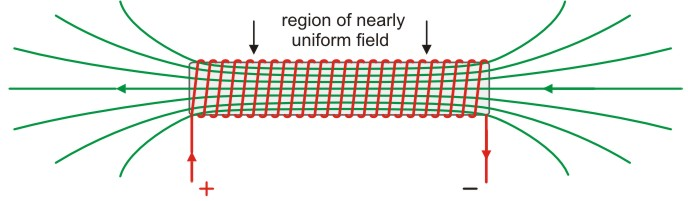
\includegraphics[height= 3cm]{fieldsol.jpg}
		\end{figure}
			\end{center}
	
	
		On the edges of the coil the magnetic field has already decreased to approximately $\frac{1}{2} \mu \frac{N}{L}I$.
		
		During the experiment the interior of the coil was also filled with a Material with Permeability constant $\mu$. Equations \ref{eq:biot} and \ref{eq:biot constant spule} change to
	
		\begin{equation}\label{eq:biot perm}
		\vec{B}(x) = \mu_r N \frac{\mu_0}{4\pi}\frac{2\pi R^2 I}{(x^2+R^2)\nicefrac{3}{2}}
		\end{equation}
	
		\begin{equation} \label{eq:biot constant spule mit perm}
		B(x) = \mu_0 \mu_r \frac{N}{L}I
		\end{equation}
	
	\subsection{Hall effect, measuring magnetic fields}
	Moving charge carriers in a magnetic field are affected by the Lorentz Force $L_z=q\vec{v}\times \vec{B}$ which moves them at an angle perpendicular to their velocity and the magnetic field, as defined by the vector product. For a current going trough a conducting material electrons are deviated to the sides, which causes a difference in electric potentials to build up in the materials as visible in the image below.
		\begin{center}
	
		\begin{figure}[h]\label{fig:hall}
		\centering
		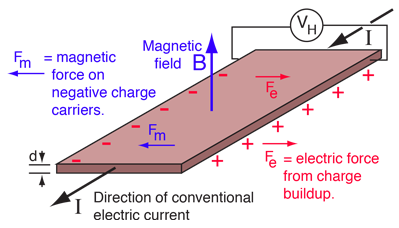
\includegraphics[height=5cm]{halleffect.jpg}
		\end{figure}
		\end{center}
	
	This effect is known as Hall effect and the difference in potential is known as Hall voltage $U_H$. This build up continues until the electric force compensates the Lorentz force
	
	\begin{equation}
		qE = q v_d B
	\end{equation}
	\begin{equation}
		E = v_dB
	\end{equation}
	\begin{equation} \label{eq:hall}
		U_h =  E w = v_d B w
	\end{equation}

	with $v_d$ being the drift velocity of the electron, w being the width of the material. By defining $A=bd$, with d being the thickness, you can rewrite the current as follows:
	\begin{equation}
		I = nqv_d A
	\end{equation}
	By using \ref{eq:hall} and solving for the charge carrier density n
	
	\begin{equation}
		n=\frac{I}{Aqv_d}=\frac{I}{bdev_d}=\frac{IB}{edU_H}
	\end{equation}
	
	So the Hall Voltage $U_H$
	\begin{equation}
		U_H=\frac{IB}{ned}=A_H\frac{IB}{d}
	\end{equation}
	With $A_H=\nicefrac{1}{ne}$ being th Hall constant of the material. By knowing this constant it is now possible to calculate the Magnetic field by measuring $U_H  $
	
	\begin{equation}
		B= \frac{U_H d}{A_H I}
	\end{equation}

	\subsection{Materials in a magnetic field}
	Depending on its reaction on an external magnetic field a material can be classified in three categories: Paramagnetic, Diamagnetic and Ferromagnetic. Para- and ferromagnets have permanent magnetic dipolmoments, that align along an external magnetic field an reinforce it. Diamagnets don't have a permanent magnetic field and they weaken the external one trough induced currents.
		\subsubsection{Paramagnetism}
		Paramagnets have permanent magnetic dipols which interactions are so weak that they align randomly. When an external magnetic field is applied the magnetic moments partially align along this field and strengthen it. $\chi_m$ is positive, temperature dependant and of te order of $10^-5$ in solid materials.
		
		\subsubsection{Diamagnetism}
		Diamagnets don't have permanent dipoles, this means that they have a closed shell for valence electrons. An external magnetic field induces currents that according to Lenz's law create a field opposing the external one and weakening it. $\chi_m$, the magnetic susceptibility is negative, temperature dependant and of te order of $10^-5$ in solid materials.
		
		\subsubsection{Ferromagnetism}
		In a ferromagnet the interactions between the magnetic dipoles is extremely big, ao that they will naturally align themselves in the same direction inside certain areas, at temperatures below $T_C$, the Curie temperature. These areas are called Weiss domains and are responsible for the magnetic characteristics of ferromagnets. These domains are separated by so called domain walls, where the magnetic dipoles' orientations changes continuously from following one domain or the other. Although these domains possess an intrinsic magnetic field, the material as a whole will not possess one since the orientations of the various domains will cause them to cancel each other out. When an external magnetic field is applied the Weiss domains which are orientated along the field grow, while others will switch direction aligning themselves with the field. This will cause the external magnetic field to increase significantly in magnitude, this means that $\chi_m$ is much bigger than 1.
		
			\begin{figure} [h] \label{fig:weiss}
			\centering
			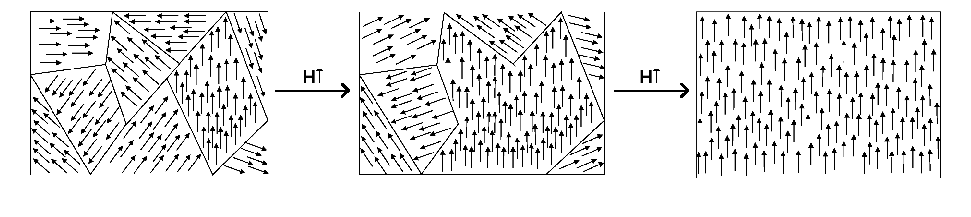
\includegraphics[height=3cm]{weiss.jpg}
			\caption{Schematic description of the process of enlargement and realignment of Weiss' domains}
		\end{figure}
		
		The magnetisation of a ferromagnet depends on the previous magnetic fields that were applied to it, since, unlike in paramagnets, the magnetisation is partly permanent. To demagnetize it heat or another magnetic field in the opposite direction in required, the so called coercive field $H_K$. The magnetisation that remains when the external field that magnetised the material is turned off is called remanence. 
		
			\begin{figure} [h]\label{fig:hyst}
			\centering
			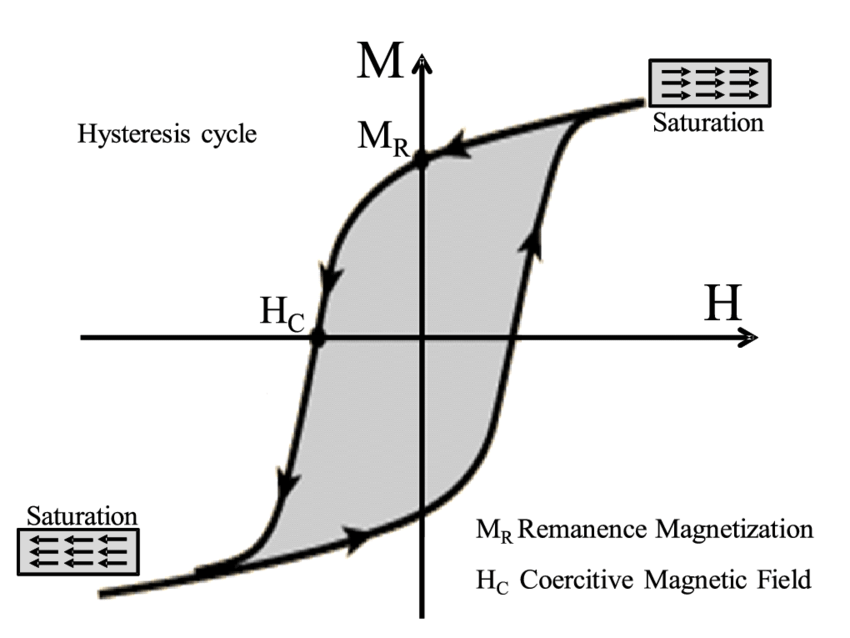
\includegraphics[height=3cm]{hysterese.jpg}
			\end{figure}
		
		
		The relationship between all the strengths of the magnetic field and the magnetisation is plotted on a hysteresis loop called main loop. As a consequence of this behavior ferromagnetic materials don't have a fixed $\chi_m$. The area inside the hysteresis curve is the energy that gets lost in heat in the processes of magnetising and demagnetising a material.
		
	\subsection{Induction} 
		A change in the magnetic flux $\Phi_m$ will induce a voltage $U_ind$. 
		\begin{equation}
		\Phi_m = \int_{A} N\vec{B}\cdot\vec{n}\,dA = \int_{A} NB_n\,dA 
		\end{equation}
	
	with $\vec{n}$ beig the normal vector to the plane A of the loop. This makes it possible to cause a change in $\Phi_m$ by changing the size or the orientation of A. the induced electromotive force is
	
	\begin{equation}\label{eq:ind}
		U_ind= -\frac{d\Phi_m}{dt}
	\end{equation}

	the minus sign being there to make it follow Lenz's rule. For the case of a coil you just need to multiply \ref{eq:ind} by N, being the number of coils.
	
		
	\section{Experimental Procedures}\label{sec:exp}
	\subsection{Instruments and Materials }
	\begin{itemize}
		\item {\bf Magnetometer}: The magnetometer has an uncertainty of 0.2\% and the probe of 0,3\%. The last digit has a $\pm1$ uncertainty. 
		\item {\bf Ruler}: the ruler has an uncertainty of 0,25\% in its scaling. The reading error is $\pm1$mm
		\item {\bf Electricity Source}: Current is measured with a multimeter with a precision of $\pm$2.5\%.
		\item {\bf Iron core} 
		\item {\bf Coil} A coil with a 3.5 cm inner radius, lenght 7.6cm and 1200 loops.
		
	\end{itemize}

	\subsection{Magnetic field along the axis of the coil (Longitudinal configuration)}
	Connect the longitudinal sensor of the magnetometer with the ruler on a sliding platform. Connect the coil with the electricity source through the multimeter. Find the maximum of the magnetic field (it will be somewhere inside the coil) and proceed to take measurements from there getting further and further away from the coil along the ruler. At every new position take a measurement of the external magnetic field. 
	Repeat this procedure 3 times in total: with 0.5A, with 1A and again with 1A but this time insert the iron core. 
	
	The maximum of the magnetic field with core will obviously be measured slightly outside of the coils, since it's the inside isn't empty.
	
	\subsection{Magnetic field in a transverse configuration} 
	Repeat the same process and measurements as for the longitudinal configuration, but this time turn the coil 90° so that its axis is perpendicular to the ruler.
	

	\section{Results and discussion}\label{sec:erg}
	\subsection{Raw data plots}
		\begin{figure}[H]\label{fig:}
			\begin{minipage}[h]{.4\linewidth}
				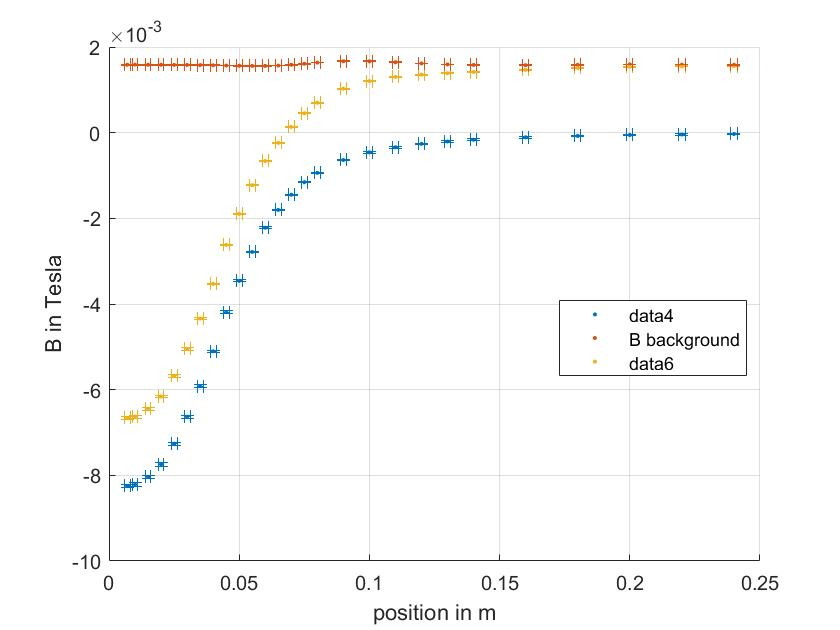
\includegraphics[height=7cm]{long 1A ohne Kern nur Punkte.jpg}
				\caption{Coil without a core, 1A, longitudinal configuration}
			\end{minipage}
			\hspace{.1\linewidth}
			\begin{minipage}[h]{.4\linewidth}
				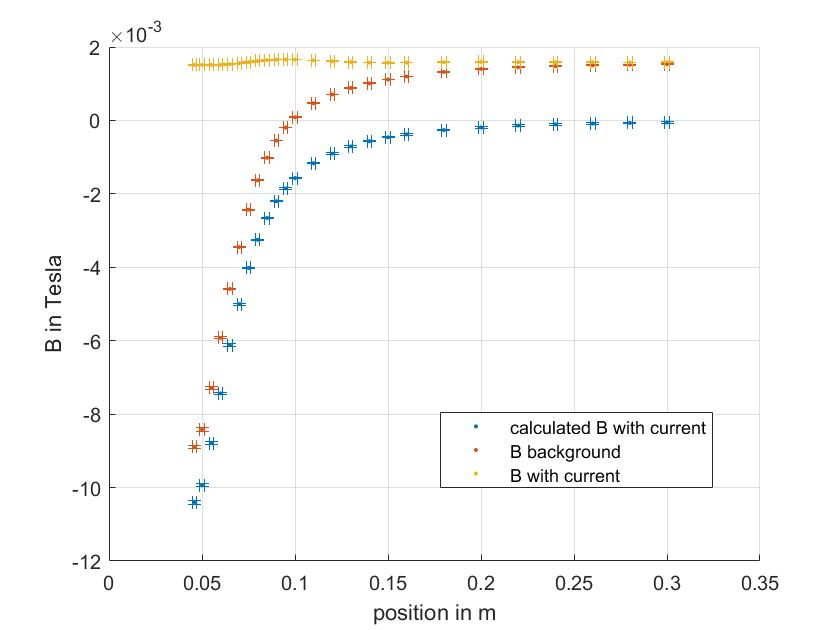
\includegraphics[height=7cm]{long 1A mit Kern nur Punkte.jpg}
				\caption{Coil with a core, 1A, longitudinal configuration}
			\end{minipage}
		\end{figure}
	
		\begin{figure}[H]
			\centering
			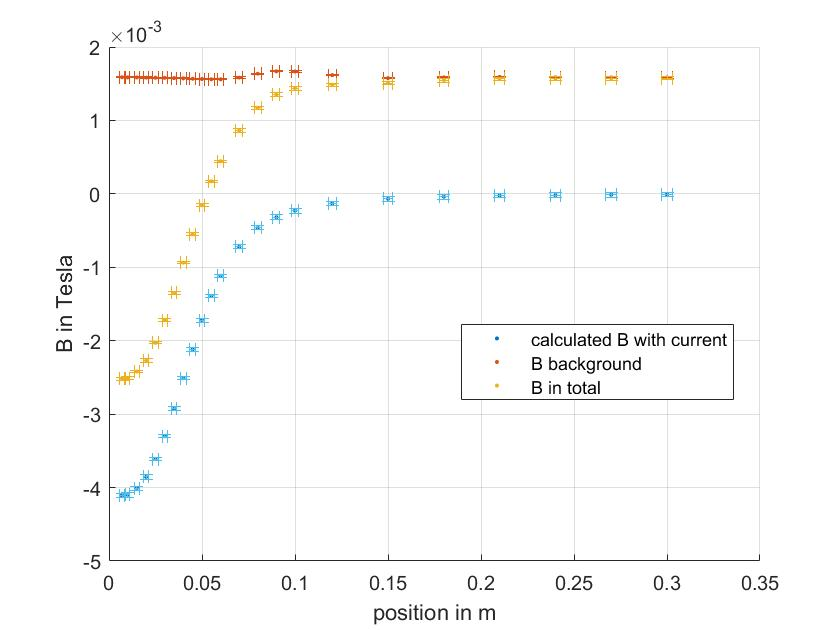
\includegraphics[height=7cm]{long 05A ohne Kern nur Punkte.jpg}
			\caption{Coil without a core, 0.5A, longitudinal configuration}
		\end{figure}
	
	\subsection{Magnetic field, without core, longitudinal configuration}
		\begin{figure}[H]
		\centering
		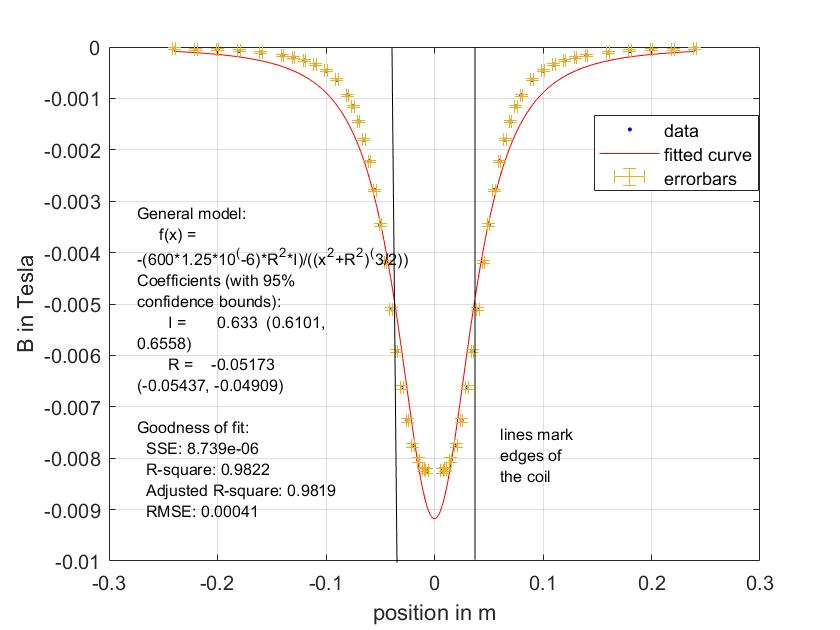
\includegraphics[height=7cm]{long 1A ohne Kern mit Spule.jpg}
		\caption{1A, mirrored magnetic field}
		\end{figure}
	As written next to the graph $I_{eff}=(0.63\pm 0.02)A$, which is a believable result since it's in the same order of magnitude as the 1A current the generator was creating and it's not greater since all the internal resistances that are unaccounted for will logically decease the current.
	$R_{eff}=(5.2\pm 0.3)cm$. The number written in the fit is negative next to the graph is negative, but since, as seen in the formula also next to the graph, R appears squared, it makes no difference so for the sake of convenience it will be treated as a positive number. Once again it's a plausible result being fairly close to the 3.5cm of inner "radius" we measured. This measure has quite a bit of uncertainty since we just measured the inner radius, not in the middle, since plastic was covering the entire coil, and the outside of the coil was also square, so instead of a radius ot was more of half a side length of a square. 
	
	\begin{figure}[H]
		\centering
		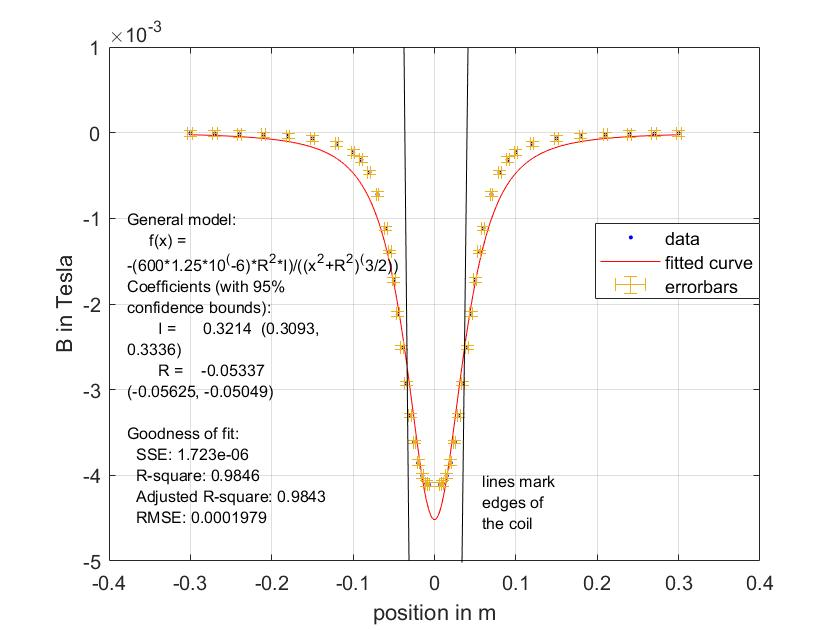
\includegraphics[height=7cm]{long 05A ohne Kern mit Spule.jpg}
		\caption{0.5A, mirrored magnetic field}
	\end{figure}
	The same considerations as above apply and if the fitting is done correctly the radius should stay the same while the current should decrease to about half, since there is a linear relationship between resistances and current. As expected $I_{eff}=(0.32\pm 0.01)A$ smaller than in the first case while $R_{eff}=(5.3\pm 0.3)cm$ stayed about the same.
	
	\subsection{Magnetic field, with core, longitudinal configuration}
	\begin{figure}[H]
		\centering
		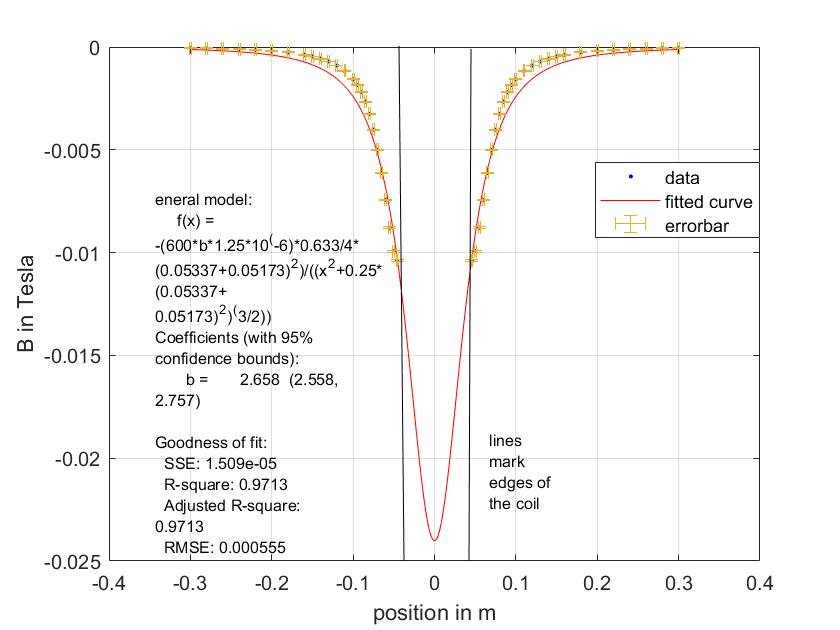
\includegraphics[height=6.8cm]{long 1A mit kern mit Spule.jpg}
		\caption{1A, mirrored magnetic field}
	\end{figure}
	The value of $\mu_r$ given by the fit is 2.658$\pm$0.1(the name of the parameter is b in the above graph) We could not pinpoint a material with this coefficient but we were able to make some guesses which we believe to be plausible. With $\mu_r$  in a range 1.003-1.05 there is Austenitic stainless steel or in a range 4-35 there is Carbonyl iron powder compound.
	The maximum of the magnetic field could not be measured because the inside of the coil had a filling. As can be read from he graph above the magnetic field inside the coil peaks at around roughly -0.024T.

	\subsection{magnetic fiel, no core, transversal configuration}
	\begin{figure}[H]
	\centering
	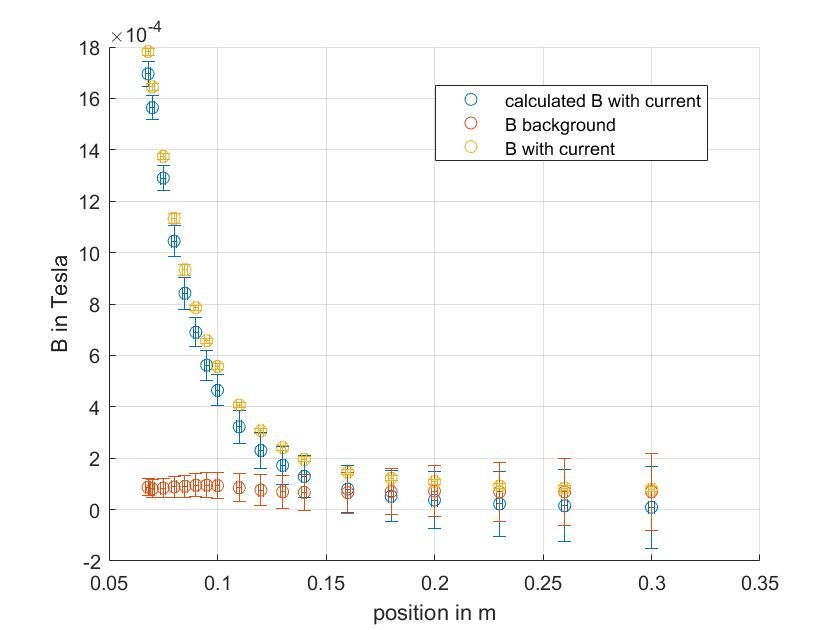
\includegraphics[height=7cm]{trans 1A mit kern nur Punkte.jpg}
	\caption{Coil without a core, 1A, transversal configuration}
	\end{figure}

	In a transverse configuration the field lines are perpendicular to the direction in which the probe is moved away from the coil. The rate at which the magnitude of the field decreases also seems to be much faster than in a longitudinal configuration. 
	
	\section{Appendix}\label{sec:anh}
		\vspace{2cm}
	\subsection{Data}
	\begin{table}[H] 
		\caption{1A, no core, longitudinal, including error}
		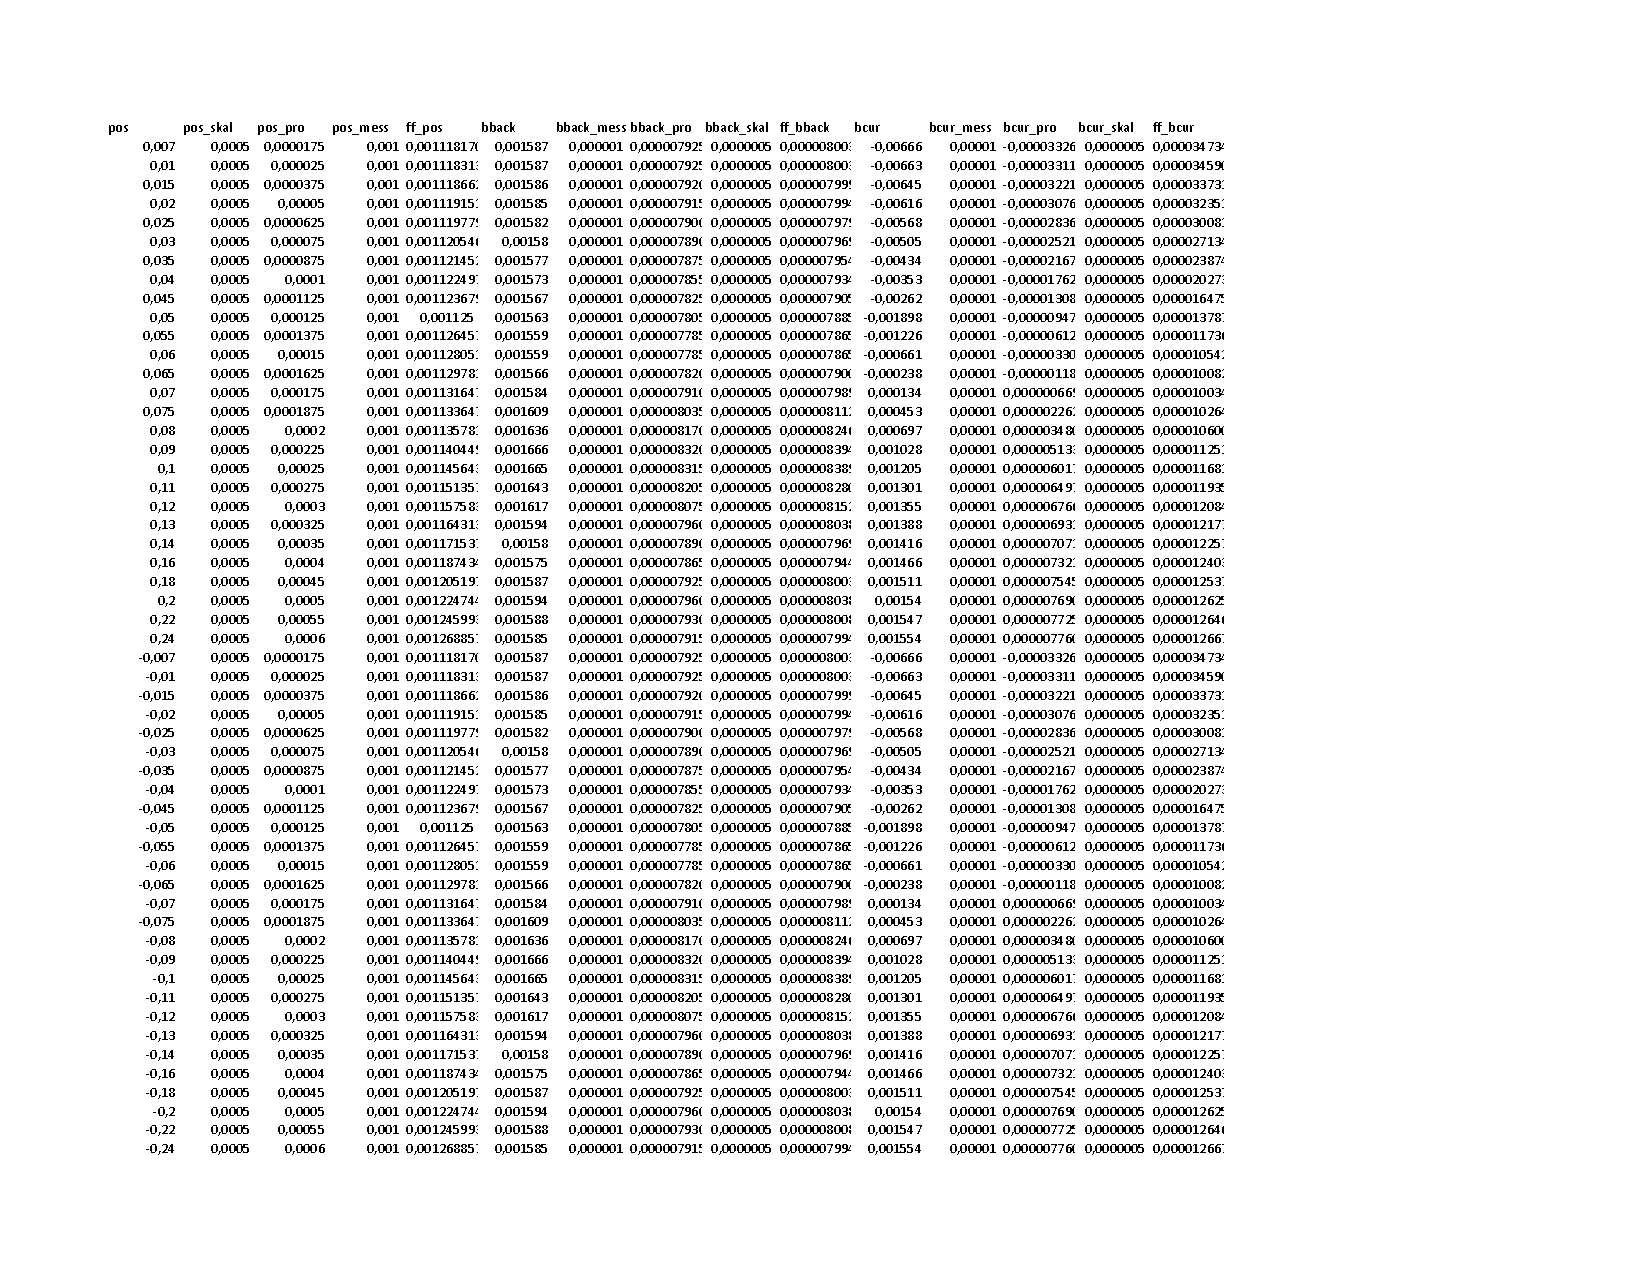
\includegraphics[width=20cm]{Daten.xlsx - 1A ohne Kern longitudinal.pdf}
	\end{table}

	\begin{table}[H]
		\caption{0.5A, no core, longitudinal, including error}
		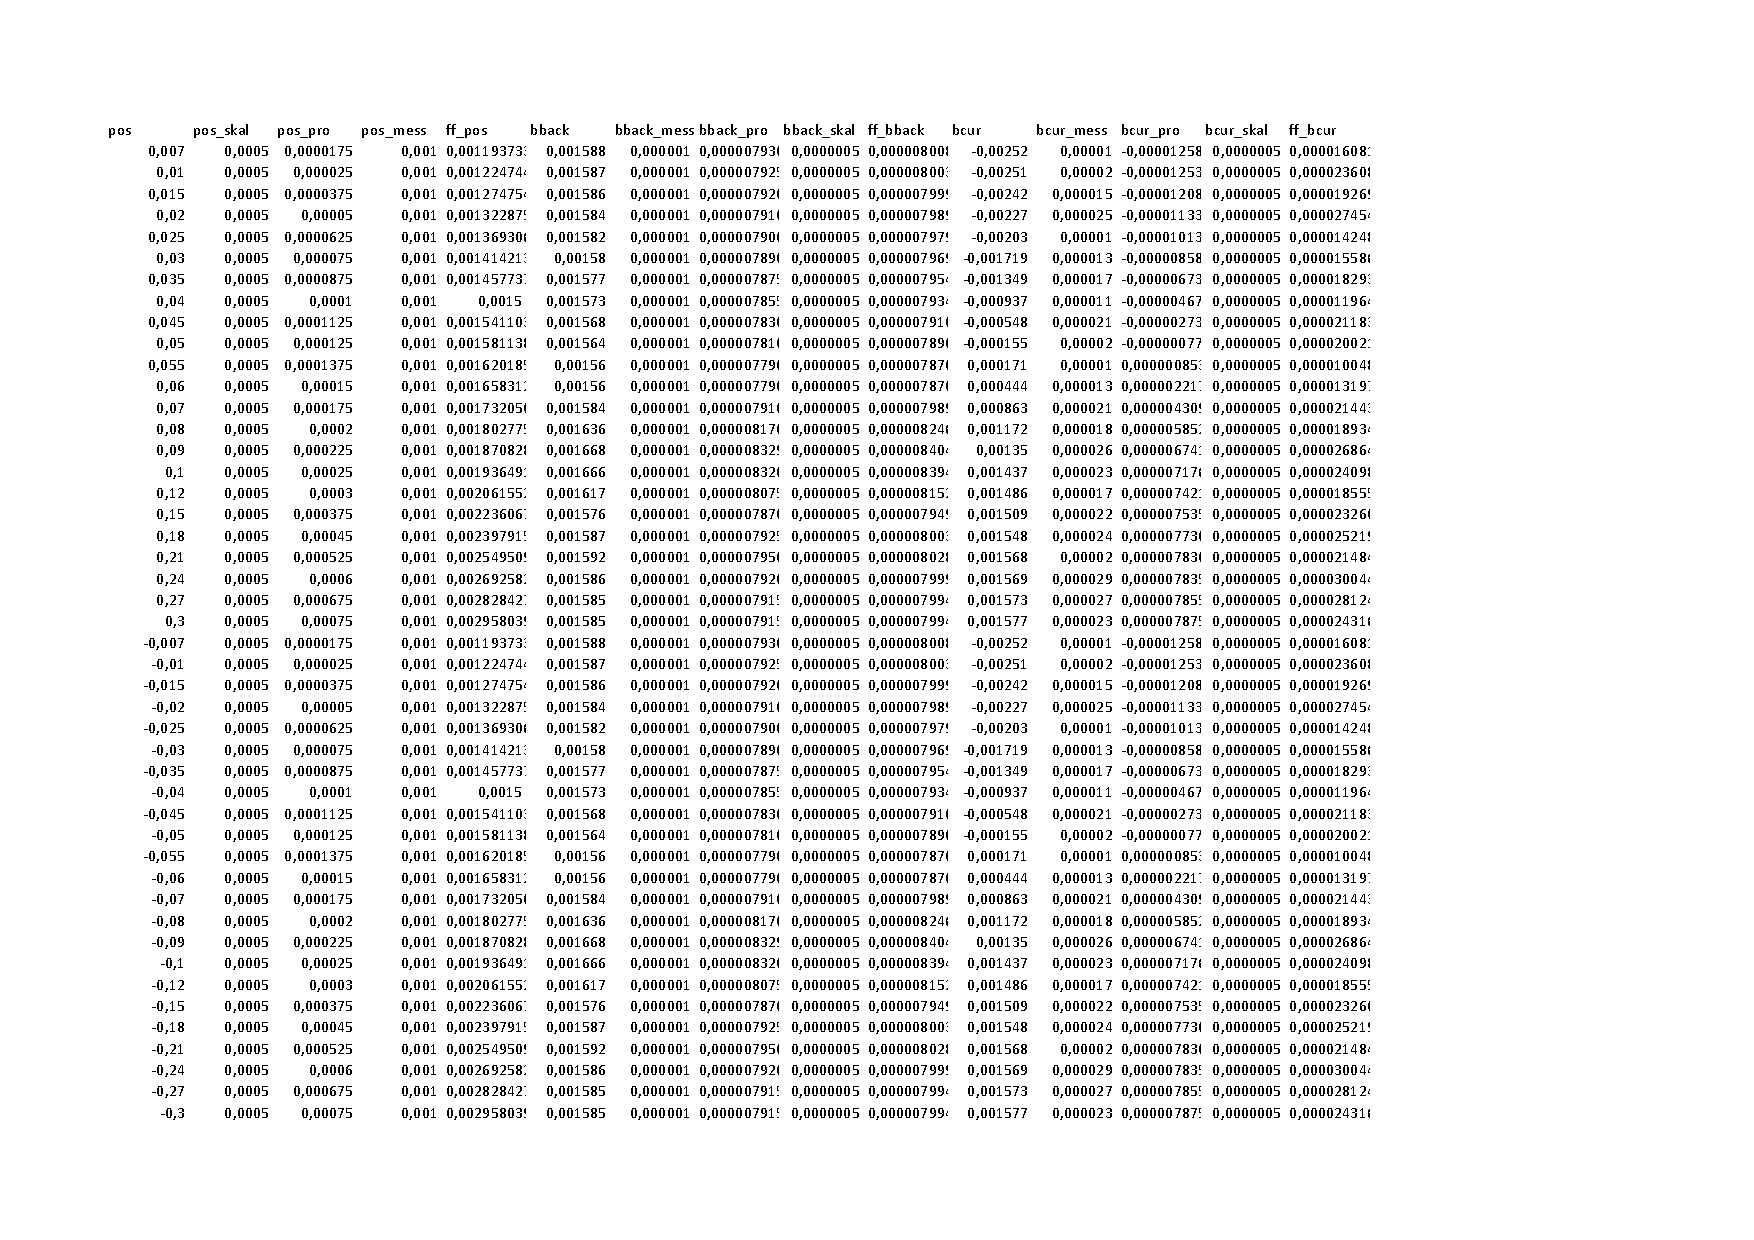
\includegraphics[width=20cm]{Daten.xlsx - 0,5A ohne Kern longitudinal.pdf}		
	\end{table}

	\begin{table}[H]
		\caption{1A, with core, longitudinal, including error}
		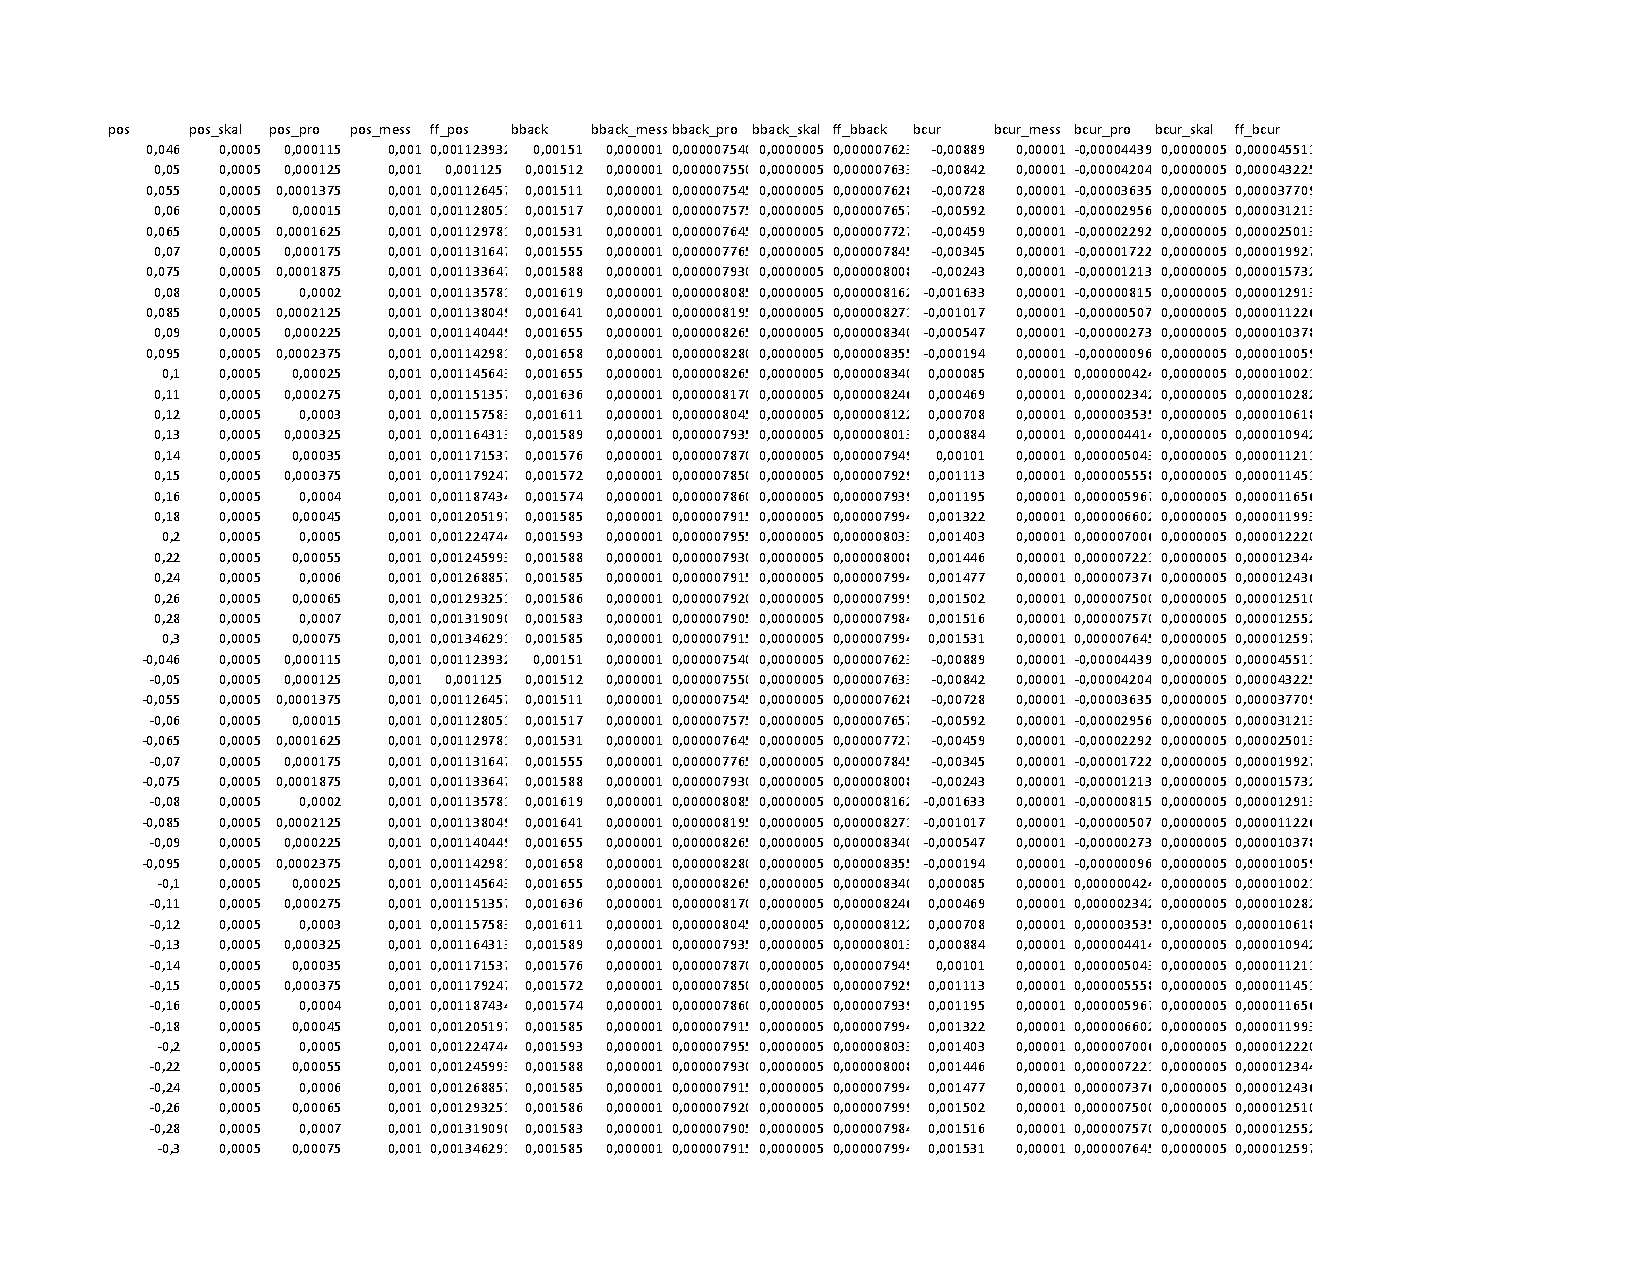
\includegraphics[width=20cm]{Daten.xlsx - 1A mit Kern longitudinal.pdf}		
	\end{table}

	\begin{table}[H]
		\caption{1A, no core, transversal, including error}
		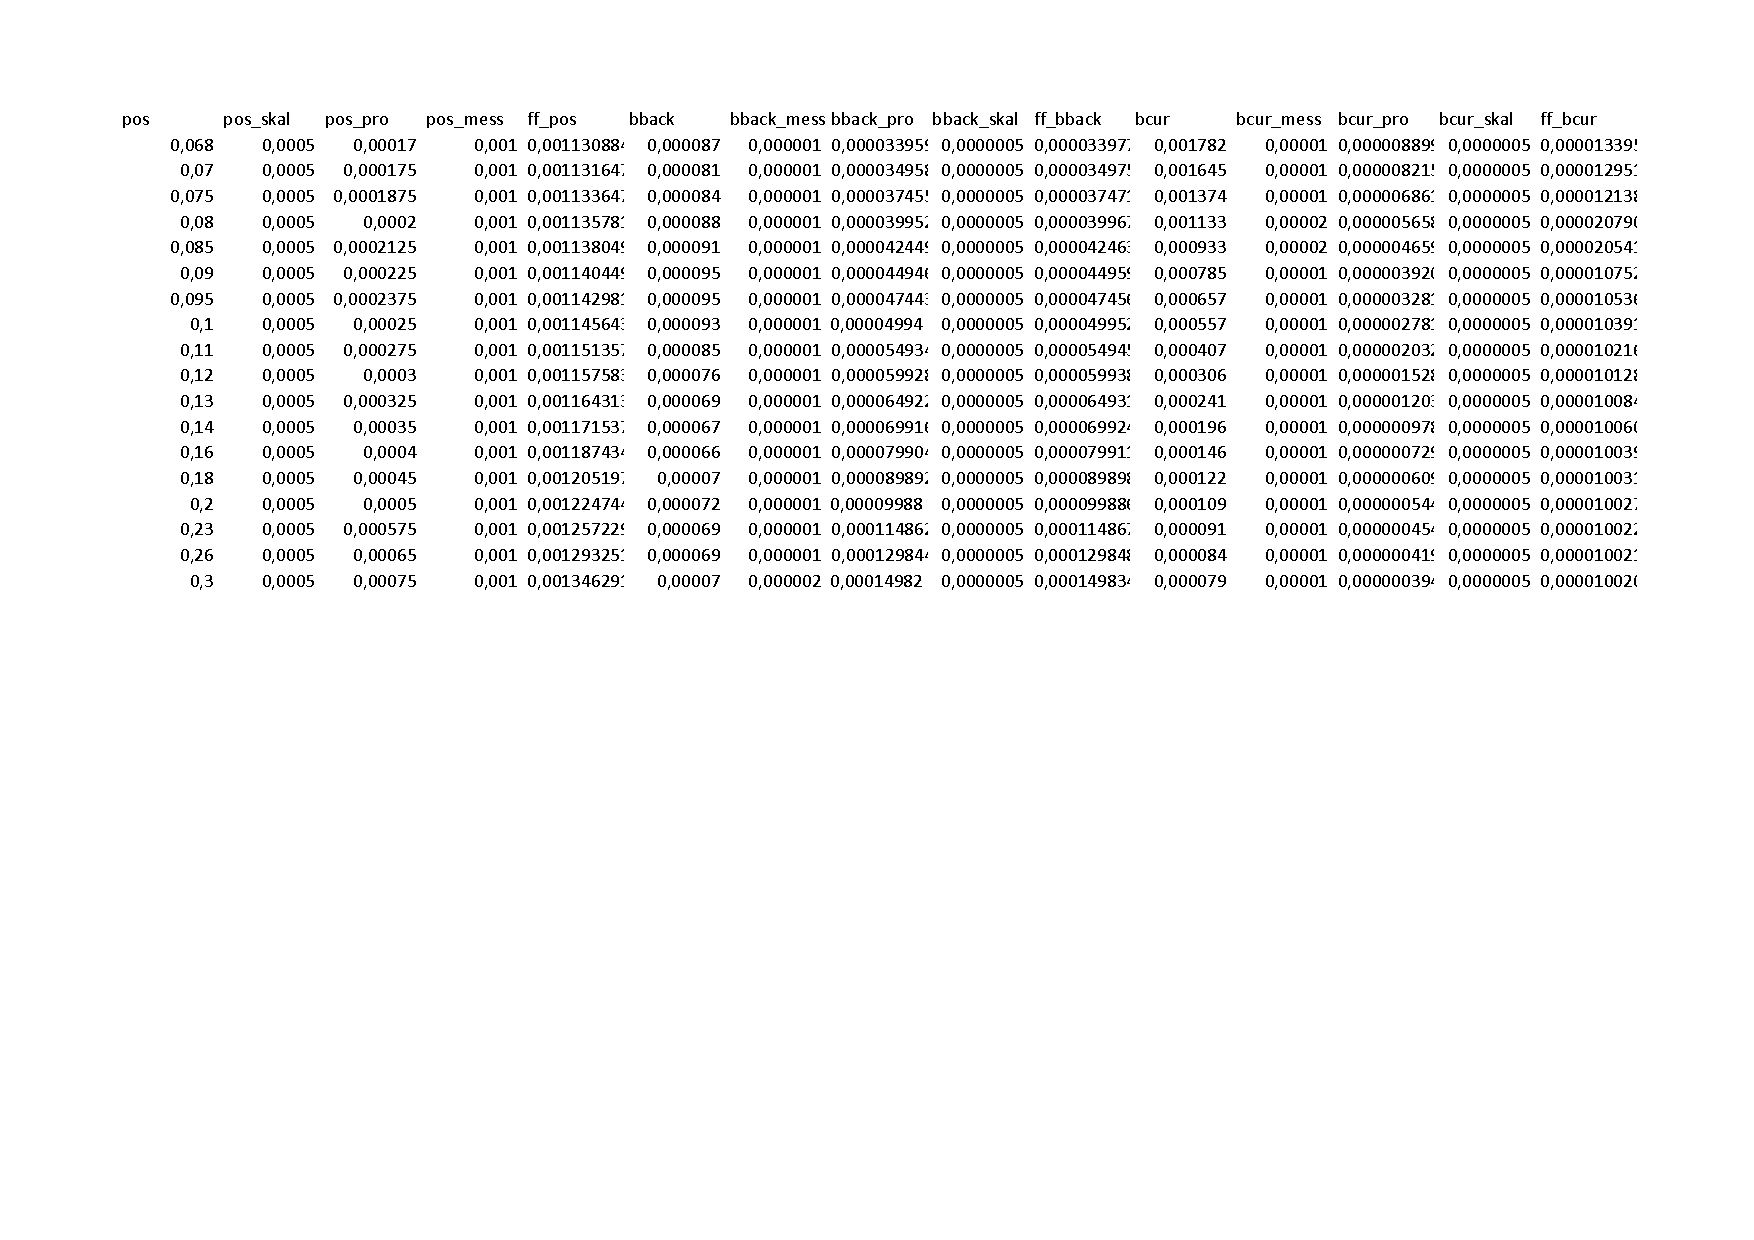
\includegraphics[width=18cm]{Daten.xlsx - 1A ohne Kern transverse.pdf}	
	\end{table}
	
	
	\subsection{Literaturverzeichnis}\label{sec:lit}
	\begin{itemize}
		\item: Wolfgang Demtröder: Elektrizität und Optik (Experimentalphysik, Bd.2); ISBN:9783540651963
		\item: https://www.ph.tum.de/academics/org/labs/ap/ap2/MAG.pdf
	\end{itemize}
	{\bf IMAGES}
	\begin{itemize}
		\item {\bf \ref{fig: Magnetisches feld spule}}: https://www.saburchill.com/physics/chapters/0046.html
		\item {\bf 	\ref{fig:hall}}: http://hyperphysics.phy-astr.gsu.edu/hbase/magnetic/Hall.html
		\item {\bf \ref{fig:hyst}}:https://www.researchgate.net/figure/Magnetic-hysteresis-in-a-ferromagnetic-material-Intercepts-points-H-C-and-M-R-are-the\_fig36\_318813955 
		\item {\bf \ref{fig:weiss}} https://physik.cosmos-indirekt.de/Physik-Schule/Weiss-Bezirk
		\item magnetic permeabilities: www.micrometals.com
		
	\end{itemize}
	\subsection{Error propagation}
	
	Gaussian error propagation from the ABW script from the internship course on Moodle was used for the error calculation. In the appendix you can find all our raw data, these are all given in SI units, which is why the values sometimes appear very small. Pos denotes the position of the measurement, Bback the background magnetic field and Bcur the magnetic field applied with a current. The resulting magnetic field B is then always B = (Bcur-Bback). In addition, you can find the directly measured errors in our data, plus the inaccuracies of the equipment (magnetometer: 0.2\%; magnetic field probe: 0.3\%; ruler: 0.25\%) and the scaling uncertainties. It is noticeable that the directly measured error in the magnetic fields is usually quite small. This is due to the fact that in most cases the display only fluctuated by $ \pm 1 $ or not at all for the last digit, only in a few exceptional cases there was a higher fluctuation.
	
	
		
		
	
	
\end{document}